\chapter{Methodology}

We conducted experiments to gain insights into the proposed methods for researching the appliance of (ND)-Laplace for cluster algorithms.
The experiment results are used to evaluate our method against other literature.
In this chapter, we explain:
\begin{enumerate}

  \item Datasets
  \item Environmental setup.
  \item For each research question: Description of the different experiments.
  \item For each research question: Results.
\end{enumerate}

\section{Research background}
\section{Research questions}

\section{Datasets} \label{datasets-section}
For this research, we selected datasets based on the related papers (\ref{theory:literature-review}).
The datasets are sourced from the UCI Machine Learning Repository \citep{noauthor_uci_nodate}.
\begin{enumerate}
  \item \textbf{Seeds dataset} \footnote{http://archive.ics.uci.edu/ml/datasets/seeds}: This dataset was used in several related works and contains 210 samples with 7 (numerical) attributes.
        The dataset contains information about seeds, like kernel width and density.
        We conducted experiments with 2, 3, and 7 dimensions and decided to use the following features (based on the correlation between the features):
        \begin{enumerate}
          \item 2-dimensional data: area and perimeter.
          \item 3-dimensional data: the kernel's area, perimeter, and length.
          \item 7-dimensional data: All numerical features.
        \end{enumerate}
  \item \textbf{Heart dataset} \footnote{https://archive.ics.uci.edu/ml/datasets/cardiotocography}: This dataset is selected because of the mixed data and amount of instances.
        It has 23 attributes, ten numerical attributes, and 2126 samples.
        The dataset contains information about measurements of fetal heart rate (FHR) and uterine contraction (UC).
        We conducted experiments with 2, 3, and 10 dimensions and decided to use the following features (based on the correlation between the features):
        \begin{enumerate}
          \item 2-dimensional data: FHR baseline and histogram-min.
          \item 3-dimensional data: FHR baseline, histogram-min, and accelerations.
          \item 10-dimensional data: All numerical features.
        \end{enumerate}
\end{enumerate}
The following datasets are for a component investigated in research question 3.
Further detail is provided in Section: \ref{method:research-question-3}.
\begin{figure}[H]
  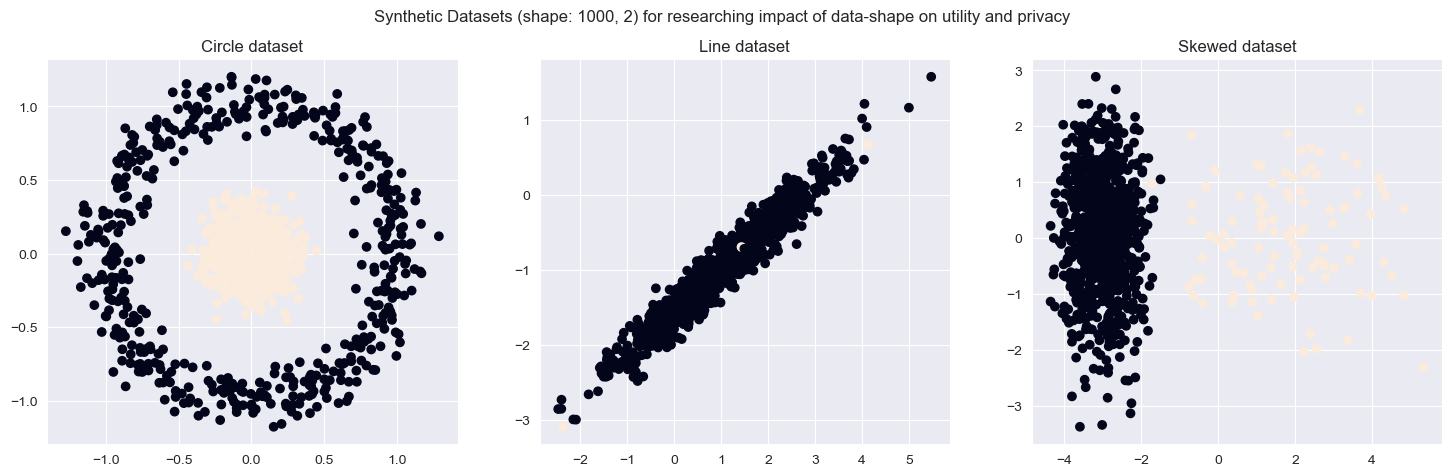
\includegraphics[width=1.0\textwidth]{Method/images/rq3.png}
  \caption{Synthetic datasets with 1000 samples and 2-dimensions}
  \label{rq3:synthetic-datasets}
\end{figure}
\begin{enumerate}
  \item \textbf{circle dataset:} Dataset with a circle shape.
  \item \textbf{line dataset:} Dataset is a line (shape is much like the seeds dataset).
  \item \textbf{skewed dataset:} Dataset samples are skewed/concentrated to one side (shape is much like the heart dataset).
\end{enumerate}
\section{Environmental setup}
For running the experiments, we use 16GB RAM and an i7-10750H 2.6Ghz processor.
The experiments are run using a Docker container which runs a pre-configured distribution of Linux Alpine.
It includes a pre-installed Anaconda environment for Python \footnote{https://github.com/devcontainers/images/tree/main/src/anaconda}\footnote{tag: mcr.microsoft.com/devcontainers/anaconda:0-3}.
We run the container using the dev-container feature for visual-studio code \footnote{https://code.visualstudio.com/docs/devcontainers/containers}.
This allows us to create a reproducible experiment environment.
\subsection{Libraries \& code versions}
We use Python version 3.9.13 with Jupyter Notebook for creating a reproducible experimental environment.
The packages for Python are:
\begin{enumerate}
  \item Scikit-learn: 1.0.*
  \item Yellow-brick: 1.5
  \item Numpy: 1.24.*
  \item Pandas: 2.0.*
  \item Seaborn: 0.11.*
  \item Mathplotlib: 3.5.*
\end{enumerate}

\section{Methods}
This section explains what methods/ algorithms we used and how we evaluate them.

\subsection{Privacy mechanisms}
We will evaluate two different privacy frameworks called kd-Laplace (our method) and piecewise (\ref{fig:piecewise-C}).
For the first one, we test three configurations/variants:
\begin{enumerate}
  \item kd-Laplace: Plain mechanism without any additions for truncation.
  \item kd-Laplace/grid: Mechanism with truncation using grid-remapping (See Equation: \ref{alg:grid-remapping-laplace}).
  \item kd-Laplace/grid/optimal: Mechanism with truncation using grid-remapping in combination with optimal-remapping (See Equation: \ref{alg:optimal-remapping-laplace}).
\end{enumerate}
The variants of kd-Laplace are different on the implementation level for 2, 3, and n-dimensional data (See figure \ref{fig:final-mechanism-design}).
Piecewise, however, will be the same for any data dimension.

We evaluate all privacy mechanisms by comparing them in utility and privacy.
To reduce the measurement bias of results, we executed them ten times for multiple privacy budgets and reported the average for each \citep{9679364}.
\begin{enumerate}
  \item The experiments run ten times, and we report the mean.
  \item All experiments run for multiple epsilons: ${0.1, 0.5, 1, 2, 3, 5, 7, 9}$.
\end{enumerate}
Firstly, we primarily focus on evaluating the utility in terms of clustering.
Then, we shift our focus to comparing the privacy mechanisms themselves.
Lastly, we compare the four mechanisms in terms of privacy.
\newpage
\subsection{Clustering methods}
For the three different algorithms: K-Means, \gls{ap}, and OPTICS, we analyzed the most important decisions regarding parameter selection (See section \ref{paragraph:choosing-r}).
This section gives a short list and explanation of the parameters we used throughout the experiments.
In addition to this, we also provide the corresponding algorithms as implemented by the Scikit-learn package.
\subsubsection{K-Means}
\begin{equation}
  \sum_{i=0}^{n}\min_{\mu_j \in C}(||x_i - \mu_j||^2)
\end{equation}
\begin{table}[h]
  \begin{tabular}{|l|p{6cm}|l|l|}
    \hline
    Parameter & Description                          & Value                                                       & Dataset        \\ \hline
    K-value   & Calculated based on an "elbow" plot. & 4 (see Figure \ref{hyperparameters:k-means-seeds-dataset})  & Seeds dataset  \\ \hline
    K-value   & ""                                   & \textbf{TODO}                                               & Heart dataset  \\ \hline
    K-value   & ""                                   & 5 (see Figure \ref{hyperparameters:k-means-circle-dataset}) & circle dataset \\ \hline
    K-value   & ""                                   & 4 (see Figure \ref{hyperparameters:k-means-line-dataset})   & line dataset   \\ \hline
    K-value   & ""                                   & 4 (see Figure \ref{hyperparameters:k-means-skewed-dataset}) & skewed dataset \\ \hline
  \end{tabular}
  \caption{K-Means hyperparameters for dataset 1 - 3}
  \label{tab:kmeans-formula-dataset-2}
\end{table}

\subsubsection{Affinity Propagation}
As specified in section \ref{theory:clustering-ap}, the clustering algorithm has two types of similarity.
The following formula calculates the responsibility:
\begin{equation}
  r(i, k) \leftarrow s(i, k) - max [ a(i, k') + s(i, k') \forall k' \neq k ]
\end{equation}
Then the availability is given using this formula:
\begin{equation}
  a(i, k) \leftarrow min [0, r(k, k) + \sum_{i'~s.t.~i' \notin \{i, k\}}{r(i', k)}]
\end{equation}
And iteratively calculated while considering the damping factor.
\begin{table}[h]
  \begin{tabular}{|l|p{6cm}|l|l|}
    \hline
    Parameter      & Description                                                                                & Value  & Dataset       \\
    \hline
    Preference     & We decided to use the median similarity as described in section \ref{theory:clustering-ap} & Median & Seeds dataset \\
    \hline
    Preference     & ""                                                                                         & Median & Heart dataset \\
    \hline

    Damping factor & Default value as specified in section \ref{theory:clustering-ap}                           & 0.5    & Seeds dataset \\
    \hline
    Damping factor & ""                                                                                         & 0.5    & Heart dataset \\
    \hline
  \end{tabular}
  \caption{Affinity Propagation hyperparameters for the datasets}
  \label{tab:ap-formula-sklearn}
\end{table}
\newpage
\subsubsection{OPTICS}
As previously explained in section \ref{theory:clustering-dbscan}, we use \gls{optics} to automatically implement \gls{dbscan} to determine the epsilon/radius.

\begin{table}[h]
  \begin{tabular}{|l|p{6cm}|l|l|}
    \hline
    Parameter      & Description                                                                                                    & Value & Dataset                       \\
    \hline
    Minimum points & Decided using the formula $minPts = n * 2$, where n is the number of features (\ref{theory:clustering-dbscan}) & 4     & Seeds dataset (2-dimensions)  \\
    \hline
    Minimum points & ""                                                                                                             & 6     & Seeds dataset (3-dimensions)  \\
    \hline
    Minimum points & ""                                                                                                             & 14    & Seeds dataset (7-dimensions)  \\
    \hline
    Minimum points & Decided using the formula $minPts = n * 2$, where n is the number of features (\ref{theory:clustering-dbscan}) & 4     & Heart dataset (2-dimensions)  \\
    \hline
    Minimum points & ""                                                                                                             & 6     & Heart dataset (3-dimensions)  \\
    \hline
    Minimum points & ""                                                                                                             & 20    & Heart dataset (10-dimensions) \\
    \hline
  \end{tabular}
  \caption{DBSCAN  hyperparameters for datasets 1 - 3}
  \label{tab:dbscan-formula-sklearn}
\end{table}

\newpage
\subsection{Utility and privacy evaluation}
\subsubsection*{Utility}
To measure cluster utility, both internal and external validation methods are used:
%Based on section \ref{theory:evaluate}, we can conclude that the corresponding literature mainly evaluates one clustering algorithm and not multiple ones.
%Furthermore, it can be concluded that if we only want to measure the coherence of the clusters, we can use an internal validation method. If we want a concrete measurement compared to the non-private version, an external validation method can be used.
%Both measurements are important to evaluate, so we use both external and internal validation. \newline
\mycomment{
  The Scikit-learn package provides the implementation for these metrics.
  With the underlying formulas:
  \begin{equation}
    AMI(U, V) = \frac{MI(U, V) - E(MI(U, V))}{avg(H(U), H(V)) - E(MI(U, V))}
  \end{equation}
  \capequation{Adjusted Mutual Information formula \citep{vinh_information_nodate-2,hubert_comparing_1985-1}}
  \begin{gather}
    RI = \frac{a + b}{C^{n}_{2}} \\
    ARI = \frac{RI - E(RI)}{max(RI) - E(RI)}
  \end{gather}
  \capequation{(Adjusted) Rand Index formula \citep{rand_objective_1971, hubert_comparing_1985-1}}
}
\begin{enumerate}
  \item \textbf{External validation: }
        The external validation is measured by comparing the labels of non-private trained cluster algorithms with those trained using a privacy mechanism.
        The outcome is between 0 and 1, where 1 indicates the highest similarity (thus the best result).
        AMI (Adjusted Mutual Information) and ARI (Adjusted Rand Index) are used to assess the external validity of the cluster algorithms (See Section \ref{theory:evaluate}).
  \item \textbf{Internal validation: }
        The internal validation measures the intrinsic properties of the clustering algorithms.
        The outcome is a value between -1 and 1 for the SC evaluation.
        Where -1 indicates incorrect clustering and 1 dense clustering.
        Another metric we use is the CH metric, where a higher value suggests good clustering (See Section \ref{theory:evaluate}).
\end{enumerate}
Because the cluster algorithms rely on Euclidean distance, we need to apply some data standardization.
For this purpose, we use standard scaling provided by the Scikit-learn package \footnote{https://scikit-learn.org/stable/modules/preprocessing.html}.

\subsubsection{Privacy}
Privacy is hard to quantify, but we can measure the privacy loss/gain by calculating the Euclidean distance between the non-perturbed and perturbed data.
In addition, we evaluate privacy by simulating a membership inference attack and calculating the adversary advantage.
\begin{enumerate}
  \item \textbf{Privacy distance: }
        The first measurement we evaluate is the distance between the dataset's non-private and private variants.
        This metric gives us a sense of how much extra distance (and privacy) the privacy mechanisms offer compared to the non-private variant.
        To this end, the average Euclidean distance is measured and reported per epsilon. A higher distance indicates more privacy.
  \item \textbf{Adversarial advantage: }
        We used the Membership Inference Attack (MIA) that Shokri et al. proposed with the implementation that was provided by Adversarial Robustness Toolkit (ART) \citep{nicolae_adversarial_2019}.
        An earlier study also explored this attack to evaluate differential privacy.
        Similar to this attack, we train a classifier with perturbed data and evaluate it using non-perturbed data (test-data / shadow-data) \citep{zhao_not_2020}.
        We consider a semi-supervised setup (figure \ref{figure:MIA-semi-supervised}), where we train a classifier with the perturbed data and evaluate it using non-perturbed data (test-data / shadow-data).
        For the classifier, we use a RandomForestClassifier \citep{rigaki_survey_2021}.
        Finally, we evaluate the adversary advantage (percentage) using $TPR - FPR$ \citep{yeom_privacy_2018}.
        Figure: \ref{figure:mi-attack} provides a visual setup of the experiment.

        Although the adversary advantage is a proven method for measuring MI attacks, we also include the TPR as an essential measurement.
        This metric is most interesting to us because this displays the percentage of the actual leaked labels (see Section \ref{theory:attack-evaluation}).
        \begin{figure}[H]
          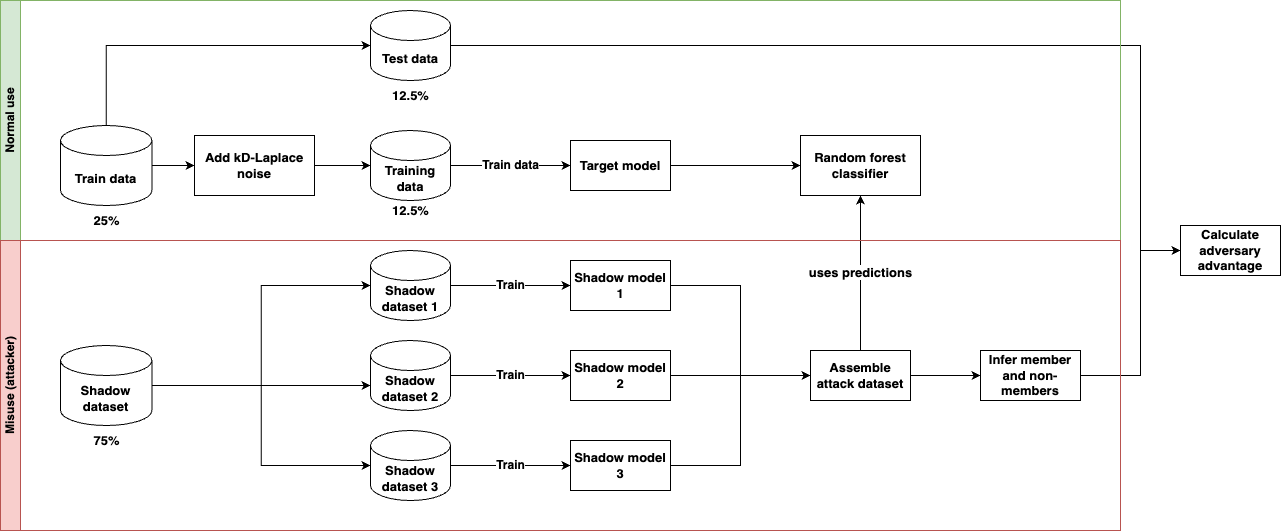
\includegraphics[width=1\textwidth]{Method/images/MI-setup.png}
          \caption{Member inference attack using shadow models. The green swim lane illustrates the normal setup, and the red swim lane projects the adversary steps.}
          \label{figure:mi-attack}
        \end{figure}
        Unlike the other utility metrics, the lower the adversary score and TPR, the better.
\end{enumerate}
\newpage
%\begin{algorithm}[H]
  \caption{Black-box inference attack}\label{alg:shokri-mi}
  \begin{algorithmic}
    \Ensure $z$
    \State $x_{target}, y_{target}, x_{shadow}, y_{shadow} = split(X)$ \Comment 75\% shadow data
    \State $x_{target-train}, y_{target-train} = split(xy_{target})$ \Comment 12.5\% train data
    \State $x_{target-test}, y_target_test = split(xy_{target})$ \Comment 12.5\% test data
    \State $Z = 2/3nD-Laplace(x_{target-train})$ 
    \State $private_classifier = RandomForestClassifier(Z, y_{target-train})$ \Comment See scikit-learn (\textbf{Bron})
    \For{three times}
      \State $dataset_{shadow} = generate_shadow_datasets$ \Comment using ART implementation
    \EndFor

  \end{algorithmic}
\end{algorithm}

%Therefore, we analyze our method according to a popular attack: Membership inference attack.
%For this purpose, we make use of a black-box Member inference attack, called "HopSkipJump" \citep{chen_hopskipjumpattack_2020,li_membership_2021}.
%This attack is evaluated using a semi-supervised setup, as proposed in this figure: \ref{fig:unsupervised-mia-attack}.
%We will make use of a decision tree model for classification but can be replaced by any other classification model.
%Both the private and non-private trained models are evaluated based on the true positive rate (TPR) and false positive rate (FPR).
%Respectively meaning, the TPR is higher if the MIA is successful and likewise the FPR if the MIA is unsuccessful.
%We hypothesize that the private model leverages a higher FPR in comparison to the non-private variant.
%Therefore, it is more convenient to apply the geo-indistinguishability as an error metric provided in \ref{eq:geo-as-an-error}.
\mycomment{
  We propose several solutions for open issues based on the theoretical framework. \newline
  \subsubsection{Choosing r: } Based on the idea of Chatzikokolakis et al. to lower the radius size if the place is crowded, we can do the same with clustering.
  For this, we could use a metric like the standard division.
  This metric does precisely this by providing the deviation from the mean:

  This metric increases based on the clutteredness of the data, which allows us to generate a radius $r$ automatically regardless of domain.
  Therefore, we depend on the reconfigurability of epsilon entirely on privacy level $l$.
  The generic standard deviation can be defined as:
  \begin{equation}
    \sigma = \sqrt{\frac{\sum{(x_i - \mu)^2}}{n}}
  \end{equation}
  The $\sigma$ being our diameter $d$, the radius $r$ is then calculated as $\frac{d}{2}$. \newline
}
\mycomment{\subsubsection{Truncation:}
  We explained the theory for truncation earlier in paragraph \ref{theory:truncation}.
  The methods proposed work correctly for a geographic map where other (historical) locations for remapping are available.

  However, it is difficult to apply this to data clustering.
  The number of data points is unknown beforehand, so we may remap to a location that is too far away.
  This way, we lose essential distance information, which hurts the clustering.
  Also, the truncation threshold is so clear (the points are outside the known 2D domain) that we do not have to rely on historical data for remapping.
  Our algorithm can be much more straightforward by re-calculating the noise until it is within the domain:
}
\mycomment{
  \begin{equation}
    T(x_{max}, x_{min}, z, x_0) \begin{cases} z &\text{if } 0 < 1 \\ T(x_{max}, x_{min}, planarLaplace(epsilon, x_0), x_0)  &\text{else} \end{cases}
  \end{equation}
}
%\begin{algorithm}
  \caption{Truncation algorithm ($T(\min, \max, x_0, z)$) for clustering with planar Laplace}\label{alg:truncaction-rq1}
  \begin{algorithmic}
    \Ensure $z$
    \State $x_1, y_1 \gets x_{min}$
    \State $x_2, y_2 \gets x_{max}$
    \State $z_x, z_y \gets z$
    \If{$x_1 < z_x < x_2$ and $y_1 < z_y < y_2$}
    \State \Return $z$
    \Else
    \State $x, y \gets x_0$
    \State $z_2 \gets LP(\epsilon, x, y)$ \Comment See formula 3.3.
    \State \Return $T(x_{min}, x_{max}, x_0, z_2)$ \Comment Rerun recursively
    \EndIf
  \end{algorithmic}
\end{algorithm}
%This algorithm uses $x_{min}$ and $x_{max}$ to re-calculate the points within the domain using respectively the minimum X/Y and maximum X/Y.
%An example of this is visualized:
%\begin{figure}[h]
%  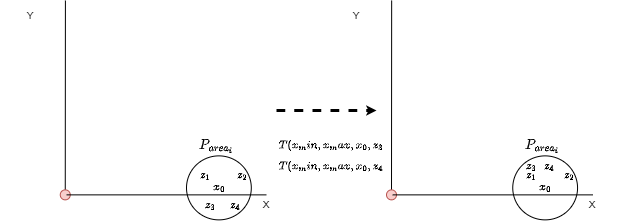
\includegraphics[width=0.8\textwidth]{Method/images/truncation-rq1.png}
%  \label{fig:truncation}
%  \centering
%  \caption{Representation of the remapping algorithm for clustering for points $z_3$ and $z_4$ }
%\end{figure}

%\subsubsection{Probability metric $K(x)(Z)$}
%\todo[inline]{Explain the probability metric $K$ we used}

%\newpage
%\subsubsection{Algorithm}
%The full algorithm for the perturbation:
%\begin{algorithm}[H]
  \caption{Full algorithm for perturbing cluster data based on planar/2D-Laplace \citep{DBLP:journals/corr/abs-1212-1984}}\label{alg:rq1}
  \begin{algorithmic}
    \Require $x \in X$  \Comment 2D array of points
    \Require $l \in R^ +$
    \Ensure $z \in Z$ \Comment 2D array of perturbed points
    \State $r = \frac{\sigma}{2}$ \Comment formula 4.1
    \State $\epsilon = \frac{l}{r}$ \Comment Calculating privacy budget \citep{DBLP:journals/corr/abs-1212-1984}
    \State $x_{min} \gets min(X)$
    \State $x_{max} \gets max(X)$
    \State $Z \gets []$
    \For{$point_i \in X$}
    \State $\theta \gets [0, \pi2]$       \Comment Random noise for $\theta$
    \State $p \gets [0, 1]$
    \State $z_i \gets C{_\epsilon}{^{-1}}(p)$       \Comment formula 3.2
    \State $z_i \gets T(x_{min}, x_{max}, point_i, z_i)$ \Comment algorithm 1.
    \State $x_{perturbed} \gets point_{i_x} + (z_{i_x} * \cos(\theta)) $ \Comment add noise to x-coordinate
    \State $y_{perturbed} \gets point_{i_y} + (z_{i_y} * \sin(\theta)) $ \Comment add noise to y-coordinate
    \State append $x_{perturbed}, y_{perturbed}$ to Z
    \EndFor
    \State \Return Z
  \end{algorithmic}
\end{algorithm}
%% We apply the theory for planar laplace proposed by \citep{DBLP:journals/corr/abs-1212-1984}

\subsection{Research question 3} \label{method:research-question-3}
%\todo[inline]{Added ideas for research question 3}
In this research question, we compare the behavior of our mechanism with what we have observed in the literature for similar mechanisms.
To do this, we have formulated several hypotheses.
\begin{enumerate}
  \item \textit{Adding optimal remapping improves utility without sacrificing privacy:}
        Since the noise is updated based on the density of the data points, the clusters stay preserved (\ref{alg:optimal-remapping-laplace}).
        As a result, the utility increases while the data points remain indistinguishable.
        Therefore, we have extended our mechanism with optimal remapping and named it kd-Laplace/grid/optimal.
        This variant is included in the next three sections and further research using the next two hypotheses.
  \item \textit{The privacy leakage (adversary advantage) increases for a higher number of dimensions:}
        The hypothesis arose from our observation while investigating/implementing kd-laplace/grid/optimal (\ref{theory:privacy-utility-nd}).
        Adding more dimensions (5 >) decreases the added noise gradually.
        The study is conducted for the kd-Laplace/grid/optimal mechanism to analyze its behavior.
  \item \textit{The shape of the data negatively impacts the kd-Laplace mechanism in terms of privacy and utility:}
        Because the mechanism heavily relies on Euclidean distance, the shape (distance between the data points) can ultimately harm utility and privacy.
        We have already observed this difference when comparing the heart and seed datasets in research questions 1 and 2.
        But, to rule out the potential impact of the number of data points (the heart dataset has 2126 samples and the seed-dataset 210), we generate three synthetic datasets, each with 1000 samples (See section \ref{datasets-section}).

\end{enumerate}
%In addition to testing the hypotheses, we also want to investigate the behavior of our mechanism in more detail.
%\begin{enumerate}
%\item Research the applicability of the mechanism for other cluster algorithms, like hierarchical clustering.
%  \item Research the impact of the data shape on privacy leakage.
%\item Explore options to extend the method to support categorical data.
%\item Explore options to extend the method to support binary data.
%\item Research possibility to include the privacy mass: \ref{equation:privacy-mass-a}.
%\end{enumerate}
